w.l.o.g we assume $B = 1$.
We denote by $O$ an optimal set. 
We denote by $x$ and $y$ the first two elements in $O$ dropped by the algorithm.  
We denote by $A$ the set of elements constructed by the algorithm just before
dropping $x$ and by $B$ the set of elements chosen by the algorithm right after dropping $x$ 
and just before dropping $y$.

\begin{figure}[h]
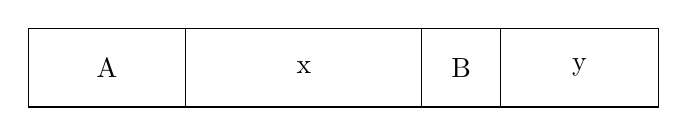
\begin{tikzpicture}[]
\draw 
	(0,0) 
	rectangle ++(2,1) node[pos=.5]{A}
 	rectangle ++(3,-1) node[pos=.5]{x}
 	rectangle ++(1,1) node[pos=.5]{B}
 	rectangle ++(2,-1) node[pos=.5]{y};
\end{tikzpicture} 
\end{figure}

Let $c(x) = 1/2 + \delta$ 
then $c(A) > 1/2 - \delta$, $c(y) \leq 1/2 - \delta$, and $c(B) \geq 2\delta$.

\begin{lemma}
Let $S$ be any set and $C$ be the set produced by the algorithm 
before dropping the first element from $S$ then $f(C) \geq (1 - e^{-\frac{c(C)}{c(S)}})f(S)$.  
\end{lemma} 

\begin{observation}
$f(A) \geq (1 - e^{\delta - 1/2})f(O)$
\end{observation}

TODO verify this $\Downarrow$
\begin{observation}
$f_A(B) \geq (1 - e^{4\delta / (2\delta - 1)})f_A(O \setminus x)$
\end{observation}

